%!TEX TX-program = xelatex
\documentclass[8pt]{article}
\usepackage{allan-eason}

\usetikzlibrary{positioning}
\usetikzlibrary{svg.path}

\graphicspath{ {./images/} }

\author{\normalfont\sffamily\large\bfseries{高一(4)班\ 邵亦成\ 48号}}
\title{\normalfont\sffamily\huge\bfseries{\textcolor{allanblue}{220406}\ \textcolor{allancyan}{三角函数(2)}\ 题目选解}}
\date{}

\geometry{a4paper, scale=0.8}

\lhead{\textcolor{allanblue}{220406}\ \textcolor{allancyan}{三角函数(2)}\ 题目选解}

\begin{document}

	\maketitle

	\section{填空题}
		\defword{1. }$y=\tan\left(\dfrac{\pi}{6}x+\dfrac{\pi}{3}\right)$的定义域为\answord{$\displaystyle \bigcup_{k\in\ZZ}\left(-5+6k, 1+6k\right)$}.
		
		\answord{解析. }三角函数的定义域.
		~\\

		\defword{2. }命题$\alpha: b=0$是命题$\beta:$函数$y=a\sin x+b\cos x$是奇函数的\answord{充分必要}条件.
		
		\answord{解析. }三角函数的广义奇偶性; 三角变换.
		~\\

		\defword{3. }$y=\tan x-\cot x$的最小正周期是\answord{$\dfrac{\pi}{2}$}.
		
		\answord{解析. }三角函数的周期性; 三角变换.
		~\\

		\defword{4. }$\displaystyle \max_{x\in\left[0, \frac{\pi}{3}\right]} 2\sin\dfrac{3}{4}x=\ansmath{\sqrt{2}}$.
		
		\answord{解析. }三角函数的极值性.
		~\\

		\defword{5. }在$\triangle ABC$中, 若$\dfrac{a}{\cos A}=\dfrac{b}{\cos B}=\dfrac{c}{\cos C}$, 则$\triangle ABC$是\answord{等边三角形}.
		
		\answord{解析. }解三角形, 三角变换.
		~\\

		\defword{6. }下列命题中正确的序号是: (1) 函数$y=\sin x$在第一象限递增; (2) 函数$y=\abs{\tan 2x}$的最小正周期为$\dfrac{\pi}{4}$; (3) 函数$y=\sin\abs{x}$的值域为$[0, 1]$; (4) 函数$y=\cos \left(\pi - \sin x\right)$是偶函数. \answord{(4)}.
		
		\answord{解析. }三角函数的性质.
		~\\
		
		\defword{7. }函数$y=\sin\left(\dfrac{x}{2}+\dfrac{\pi}{4}\right), x\in \left[-2\pi, 2\pi\right]$的递增区间是\answord{$\left[-\dfrac{3}{2}\pi, \dfrac{1}{2}\pi\right]$}.
		
		\answord{解析. }三角函数的单调性.
		~\\

		\defword{8. }在$\triangle ABC$中, 若$\angle A=120\degree, AB=5, BC=7$, 则$S_{\triangle ABC}=\ansmath{\dfrac{15\sqrt{3}}{4}}$.
		
		\answord{解析. }解三角形.
		~\\

		\defword{9. }函数$f(x)=A\sin(\omega x+\varphi) (A, \omega, \varphi$是常数$, A>0, \omega > 0)$的部分图像如图所示, 则$f(0)=\ansmath{\dfrac{\sqrt{6}}{2}}$.

		$$
			\begin{tikzpicture}[scale = 1.5, baseline = 0]
				\draw[black, ->] (-0.75, 0)--(3, 0) node[below] {$x$} node at ({pi/3}, 0)[anchor = south west] {$\dfrac{\pi}{3}$};
				\draw[black, ->] (0, -2)--(0, 2) node[right] {$y$};
				\draw[black, domain = -1 : 3, samples = 2000] plot(\x, {sqrt(2) * sin(deg(2 * \x + pi / 3))});
				\draw[black, dashed] ({1 / 12 * pi}, {sqrt(2)})--(0, {sqrt(2)}) node[left] {$\sqrt{2}$};
				\draw[black, dashed] ({7 / 12 * pi}, {-sqrt(2)})--(0, {-sqrt(2)}) node[left] {$-\sqrt{2}$};
				\draw[black, dashed] ({7 / 12 * pi}, {-sqrt(2)})--({7 / 12 * pi}, {0}) node[above] {$\dfrac{7}{12}\pi$};
			\end{tikzpicture}
		$$
		
		\answord{解析. }形如$f(x)=A\sin(\omega x+\varphi)+B$的函数图像的性质.
		~\\
		
		\defword{10. }$E, F$是等腰$\Rt \triangle ABC$斜边$AB$上的三等分点, 则$\tan \angle ECF=\ansmath{\dfrac{3}{4}}$.

		$$
			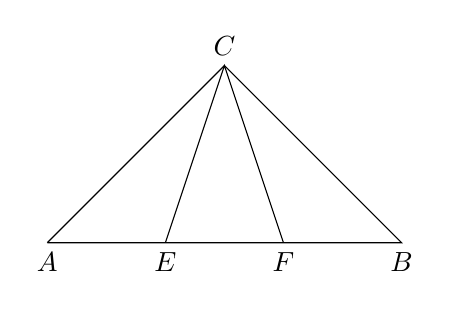
\begin{tikzpicture}[scale = 1.5, baseline = 0]
				\draw[black] (0, 0)--(3, 0)--(1.5, 1.5)--(0, 0) node at (0, 0) [anchor = north] {$A$} node at (3, 0) [anchor = north] {$B$} node at (1.5, 1.5) [anchor = south] {$C$};
				\draw[black] (1, 0)--(1.5, 1.5)--(2, 0) node at (1, 0) [anchor = north] {$E$} node at (2, 0) [anchor = north] {$F$};
			\end{tikzpicture}
		$$
		
		\answord{解析. }解三角形.
		~\\

		\defword{11. }在$\triangle ABC$中, $a^2 - b^2 = \sqrt{3} bc$, $\sin C = 2\sqrt{3} \sin B$, 则$A=\ansmath{\dfrac{\pi}{6}}$.
		
		\answord{解析. }解三角形, 三角变换.

		$$\sin C = 2\sqrt{3} \sin B \Rightarrow c=2\sqrt{3} b,$$

		有

		\begin{align*}
			\cos A &= \frac{b^2 + c^2 - a^2}{2bc}\\
			       &= \frac{c^2 - \sqrt{3} bc}{2bc}\\
			       &= \frac{c - \sqrt{3}b}{2b}\\
			       &= \frac{2\sqrt{3}b - \sqrt{3}b}{2b}\\
			       &= \frac{\sqrt{3}}{2},
		\end{align*}

		故有\answord{$A=\dfrac{\pi}{6}$}.
		~\\

		\defword{12. }在$\triangle ABC$中, $a^2 - c^2 = 2b$, $\sin A \cos C = 3 \cos A \sin C$, 则$b=\ansmath{4}$.
		
		\answord{解析. }解三角形, 三角变换.

		\begin{align*}
			\sin A \cos C = 3\cos A \sin C &\Rightarrow a \cdot \frac{a^2+b^2-c^2}{2ab}=3c\cdot\frac{b^2+c^2-a^2}{2bc}\\
			&\Rightarrow 2(a^2-c^2)=b^2\\
			&\Rightarrow 4b=b^2\\
			&\Rightarrow \ansmath{b=4}.
		\end{align*}

	\section{解答题}
		\defword{13. }研究与函数$f(x)=\tan x$相关的问题并填写结论.
			
			\begin{enumerate}[label=(\arabic*)]
				\item 求$f\left(\dfrac{\pi}{3}-2x\right)$的定义域. \answord{$\left\{x|x\neq \dfrac{\pi}{3}-\dfrac{k}{2}\pi, k\in\ZZ\right\}$}.

				\item 求$f\left(x-\dfrac{\pi}{2}\right)$在区间$\left[-\dfrac{\pi}{4}, \dfrac{\pi}{4}\right]$之间的值域. \answord{$(-\infty, -1]\cup[1, +\infty)$}.

				\item 求函数$f\left(\dfrac{\pi}{3}-2x\right)$与$\abs{f(x)}$的周期. \answord{$T\in\left\{T|T=\dfrac{k\pi}{2}, k\in \ZZ, k\neq 0\right\}, T\in\left\{T|T=k\pi, k\in \ZZ, k\neq 0\right\}$}.

				\item 写出函数$f\left(\dfrac{\pi}{3}-2x\right)$的单调区间并指明增减. \answord{单调减: $\displaystyle \left(\dfrac{k\pi}{2} + \dfrac{5}{12}\pi, \dfrac{k\pi}{2} + \dfrac{11}{12}\pi\right), k\in \ZZ$}.

				\item 写出$f(2x)$图像的所有对称中心. \answord{$P\left(\dfrac{k\pi}{4} + \dfrac{\pi}{4}, 0\right), k\in\ZZ$}.
			\end{enumerate}

		\answord{解析. }三角函数的性质.
		~\\

		\defword{14. }如图, 位于$A$处的信息中心获悉: 在其正东方向相聚$40$海里的$B$处有一艘渔船遇险, 在原地等待营救. 信息中心立即把消息告知在其南偏西$30\degree$, 相距$20$海里的$C$处的乙船, 现乙船向北偏东$\theta$的地方沿直线$CB$前往$B$处救援, 求$\cos \theta$.

		$$
			\begin{tikzpicture}[scale = 0.2, baseline = 0]
				\draw[black, ->] (-20, 0)--(50, 0) node [below] {东} node at (20, 0) [anchor = south] {$40$};
	    		\filldraw[black] (0, 0) circle (1em) node[anchor = south east] {$A$};
	    		\filldraw[black] (40, 0) circle (1em) node[anchor = north] {$B$};
				\draw[black, ->] (0, -30)--(0, 10) node [above] {北};
				\draw[black] (0, 0)--(-10, {-10 * sqrt(3)}) node at (-5, {-5 * sqrt(3)}) [anchor = south east] {$20$};
	    		\filldraw[black] (-10, {-10 * sqrt(3)}) circle (1em) node[anchor = north] {$C$};
	    		\draw[black] (0, -3) arc[start angle = 270, end angle = 240, radius = 3] node at (-1.5, -5) [anchor = north] {$30\degree$};
	    		\draw[black, dashed] (-10, {-10 * sqrt(3)})--(40, 0);
	    		\draw[black, dashed] (-10, {-10 * sqrt(3)})--(-10, 0) node[above] {$Q$};
	    		\draw[black] (-7, 0)--(-7, -3)--(-10, -3);
	    		\draw[black] (-10, {-10 * sqrt(3) + 5}) arc[start angle = 90, end angle = {90 - 70.89339465}, radius = 5] node at (-7, {-8 * sqrt(3)}) [anchor = south west] {$\theta$};
			\end{tikzpicture}
		$$

		\answord{解析. }初中数学.

		联结$CB$, 作$CQ \perp BA$于$Q$. 显然有$QA=10 (\mathrm{nm}), QC=10\sqrt{3} (\mathrm{nm}), \angle QCB = \theta$. 有$\cos \theta = \dfrac{CQ}{CB}$, 而$CQ = 10\sqrt{3}, CB = \sqrt{(40 + 10)^2 + (10\sqrt{3})^2}$, 则有$\cos \theta = \dfrac{\sqrt{21}}{14}$
		~\\

		\defword{15. }在$\triangle ABC$中, $A, B, C$为三内角, $f(B) = 4 \cos B \sin^2 \left(\dfrac{\pi}{4} + \dfrac{B}{2}\right) + \sqrt{3} \cos 2B - 2 \cos B$,

		\begin{enumerate}[label=(\arabic*)]
			\item 若$f(B)=2$, 求$B$.

				\answord{解析. }三角方程, 三角变换.

				\begin{align*}
					f(B) &= 4\cos B \sin^2 \left(\dfrac{\pi}{4}+\dfrac{B}{2}\right) + \sqrt{3} \cos 2B - 2 \cos B\\
					     &= 2 \cos B \sin B + \sqrt{3} \cos 2B\\
					     &= 2\sin \left(2B + \dfrac{\pi}{3}\right).
				\end{align*}

				$$f(B) = 2 \Rightarrow 2\sin \left(2B + \dfrac{\pi}{3}\right) = 2 \Rightarrow \ansmath{B = \dfrac{\pi}{12}}.$$

			\item 若$f(B)-m > 2$恒成立, 求实数$m$的取值范围.

				\answord{解析. }三角不等式, 三角变换.

				$$f(B)-m>2 \Iff 2\sin \left(2B + \dfrac{\pi}{3}\right) > 2+m,$$

				\begin{align*}
					0 < B < \pi &\Rightarrow -2 \leq 2\sin \left(2B + \dfrac{\pi}{3}\right) \leq 2\\
					&\Rightarrow 2+m < -2\\
					&\Rightarrow \ansmath{m<-4}.
				\end{align*}

		\end{enumerate}

	\section{附加题}
		\defword{16. }如图, 某园林单位准备绿化一块直径为$BC$的半圆形空地, $\triangle ABC$外的地方种草, $\triangle ABC$的内接正方形$PQRS$为一水池, 其余的地方种花. 若$BC=a, \angle ABC=\theta$. 设$S_{\triangle ABC} = S_1, S_{PQRS} = S_2$,

		$$
			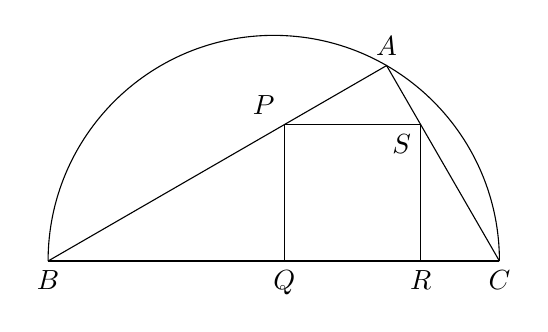
\begin{tikzpicture}[scale = 1, baseline = 0]
				\draw[black] ({(3 + sqrt(3) + 1)}, 0) arc[start angle = 0, end angle = 180, radius = {(3 + sqrt(3) + 1) / 2}];
				\draw[black] (0, 0) -- ({(3 + sqrt(3) + 1)}, 0) node at (0, 0) [anchor = north] {$B$} node at ({(3 + sqrt(3) + 1)}, 0) [anchor = north] {$C$};
				\draw[black] (3, 0) -- (3, {sqrt(3)}) -- ({3 + sqrt(3)}, {sqrt(3)}) -- ({3 + sqrt(3)}, {0}) node at (3, 0) [anchor = north] {$Q$} node at ({3 + sqrt(3)}, 0) [anchor = north] {$R$};
				\draw[black] (0, 0) -- ({3 * (3 + sqrt(3) + 1) / 4}, {sqrt(3) * (3 + sqrt(3) + 1) / 4}) -- ({(3 + sqrt(3) + 1)}, 0) node at ({3 * (3 + sqrt(3) + 1) / 4}, {sqrt(3) * (3 + sqrt(3) + 1) / 4}) [anchor = south] {$A$} node at (3, {sqrt(3)}) [anchor = south east] {$P$} node at ({3 + sqrt(3)}, {sqrt(3)}) [anchor = north east] {$S$};
			\end{tikzpicture}
		$$

		\begin{enumerate}[label=(\arabic*)]
			\item 用$a, \theta$表示$S_1$和$S_2$.

				\answord{解析. }初中数学.

				$\ansmath{S_1}=\dfrac{1}{2}AB\cdot AC=\dfrac{1}{2}a\sin \theta a\cos \theta \ansmath{= \dfrac{1}{2} a^2 \sin \theta \cos \theta}. PS = \dfrac{a\sin \theta \cos \theta}{1 + \sin \theta \cos \theta}, \\\ansmath{S_2}=PS^2\ansmath{=\dfrac{a^2 \sin^2 \theta \cos^2 \theta}{1 + \sin^2 \theta \cos^2 \theta + 2\sin \theta \cos \theta}}.$

				

			\item 当$a$固定, $\theta$变化时, 求$\dfrac{S_1}{S_2}$取最小值的$\theta$.

				\answord{解析. }三角函数的极值; 三角变换, 基本不等式.

				$$\frac{S_1}{S_2}=\frac{1}{2}\cdot\frac{(1+\sin\theta\cos\theta)^2}{\sin \theta \cos \theta}=\frac{1}{\sin 2\theta} + \frac{1}{4} \sin 2\theta + 1.$$

				$t \ddef \sin 2\theta, $又$0 < \theta < \dfrac{\pi}{2},$有$t\in(0, 1],$

				$$\min \frac{S_1}{S_2} = \min_{t\in(0, 1]}\left(\frac{1}{t} + \frac{1}{4} t + 1\right) = \dfrac{9}{4}, \Iff \sin 2\theta = 1 \Leftrightarrow \ansmath{\theta = \dfrac{\pi}{4}}. $$

		\end{enumerate}

\end{document}